\documentclass[11pt]{article}
\usepackage{amsmath}
\usepackage{graphicx}
\usepackage{hyperref}
\usepackage[utf8]{inputenc}
\usepackage[spanish]{babel}
\usepackage[margin=2cm]{geometry}
\usepackage{amsfonts}
\usepackage{listings}
\usepackage[T1]{fontenc}
\usepackage{float}

\title{Ejercicio Guiado - Mineria de Flujo de Datos.}
\author{Néstor Rodríguez Vico. DNI: 75573052C - \href{mailto:nrv23@correo.ugr.es}{nrv23@correo.ugr.es}}
\date{\today}


\lstdefinestyle{bash_style}{
	language=bash,
	frame=single,
	xleftmargin=.25in,
	upquote = true,
	basicstyle=\scriptsize,
	breakatwhitespace=false,         
	breaklines=true,                 
	captionpos=b,                    
	keepspaces=true,                 
	numbers=left,                    
	numbersep=5pt,                  
	showspaces=false,                
	showstringspaces=false,
	showtabs=false,                  
	tabsize=2
}

\lstset{style=bash_style}

\begin{document}
\maketitle

\setlength{\belowdisplayskip}{5pt} 
\setlength{\belowdisplayshortskip}{5pt}
\setlength{\abovedisplayskip}{5pt} 
\setlength{\abovedisplayshortskip}{5pt}

\section{Clasificación. Ejercicio 1.}

Se pide comparar la eficacia de un Hoeffding Tree con un clasificador, para un flujo de datos de 1.000.000 de instancias generadas con un generador RandomTreeGenerator, suponiendo una frecuencia de muestreo de 10.000 y con el método de evaluación Interleaved Test-Then-Train. \\

Para \textit{Hoeffding Tree} usaremos la siguiente orden:

\begin{lstlisting}[language=bash]
java -cp moa.jar moa.DoTask "EvaluateInterleavedTestThenTrain -l trees.HoeffdingTree \
	-i 1000000 -f 10000"
\end{lstlisting}

Para \textit{Na\"{i}ve Bayes} usaremos la siguiente orden:

\begin{lstlisting}[language=bash]
java -cp moa.jar moa.DoTask "EvaluateInterleavedTestThenTrain -l bayes.NaiveBayes -i 1000000 \
	-f 10000"
\end{lstlisting}

Para saber si hay diferencias significativas, tendríamos que generar una población de resultados y escoger una medida de eficacia para comparar. Para ello, escogeremos 30 semillas diferentes y ejecutaremos 30 veces el mismo método (en total 30 ejecuciones para Na\"{i}ve Bayes y otras 30 para Hoeffding Trees). Escogeremos los resultados del porcentaje de aciertos en la clasificación, y las compararemos con un test estadístico. \\

Para agilizar este proceso, he hecho un pequeño script qie ejecuta un orden 30 veces y guarda los resultados en los \textit{csv} correspondientes. Dicho script es el siguiente:

\begin{lstlisting}[language=bash]
for i in $(seq 30)
do
	java -cp moa.jar -javaagent:sizeofag-1.0.0.jar moa.DoTask "..." \
	"-s (generators.RandomTreeGenerator -i $i)" > "$i.csv"
done
\end{lstlisting}

Sólo debemos cambiar los tres puntos de la línea 3 por la orden que queramos ejecutar. Primero lo haremos para Hoeffding Tree y luego Na\"{i}ve Bayes. Una vez tenemos los resultados de las 30 ejecuciones de cada modelo, podemos aplicar los tests estadísticos. Para ello, he usado el siguiente código en R:

\begin{lstlisting}[language=R]
read.data <- function(folder) {
	# Listamos los ficheros
	ficheros <- list.files(path = folder, full.names=TRUE)
	# Leemos los conjuntos de datos
	data <- lapply(ficheros, read.csv)
	# Tal y como dice la transparencia 19, nos quedamos el ultimo valor de 
	# la columna Classification Correct (Percent).
	sapply(data, function(x) x[nrow(x), 5])
}

naive_bayes <- read.data(folder = "naive_bayes")
hoeffding_tree <- read.data(folder = "hoeffding_tree")

shapiro.test(naive_bayes)$p.value
shapiro.test(hoeffding_tree)$p.value
tseries::jarque.bera.test(naive_bayes)$p.value
tseries::jarque.bera.test(hoeffding_tree)$p.value
t.test(naive_bayes, hoeffding_tree)$p.value

mean(naive_bayes)
mean(hoeffding_tree)
\end{lstlisting}

Tras llamarlo, los resultados obtenidos son los siguientes:

\begin{table}[H]
	\centering
	\begin{tabular}{rl}
		\textbf{Test} & \textbf{Resultado} \\ \hline
		p.value de shapiro para naive\_bayes & 0.6478472 \\
		p.value de shapiro para hoeffding\_tree & 0.8852122 \\
		p.value de jarque.bera para naive\_bayes & 0.6805229 \\
		p.value de jarque.bera para hoeffding\_tree & 0.8924791 \\
		p.value de t.test & 1.206664e-101 \\
		media de naive\_bayes & 73.67307 \\
		media de hoeffding\_tree & 94.54905
	\end{tabular}
\end{table}

Los resultados de los tests estadísticos (saphiro y jarquebera) indican que los datos siguen una distribución normal y que, por lo tanto, podemos aplicar un test paramétrico, como es el test de Student. Tras aplicarlo, podemos afirmar que hay diferencias significativas entre ambos algoritmos. Por eso, he calculado la media para ambos algoritmos y, efectivamente, Hoeffding tiene un \textit{94.54905\%} de acierto mientras que Na\"{i}ve Bayes sólo un \textit{73.67307\%}.

\section{Concept drift.}

\subsection{Ejercicio 2.}

Se pide generar 100.000 instancias utilizando el generador de datos SEAGenerator, con un desvío de concepto centrado en la instancia 20.000 en una ventana de 100 instancias. Para simular el desvío de concepto, hacer que el simulador genere la función -f 2 al principio, y luego la función -f 3. \\ Usar un clasificador Na\"{i}ve Bayes evaluado con una frecuencia de muestreo de 1.000 instancias, usando el método prequential para evaluación. Inserte la configuración directamente en la GUI de MOA para visualizar la gráfica de la evolución de la tasa de aciertos (medida accuracy). ¿Qué se observa? \\

Para solucionar este ejercicio, el comando usado en MOA es el siguiente:

\begin{lstlisting}[language=bash]
EvaluatePrequential -l bayes.NaiveBayes
	-s (ConceptDriftStream 
		-s (generators.SEAGenerator -f 2) 
		-d (generators.SEAGenerator -f 3) 
		-p 20000 -w 100)
	-i 100000 -f 1000
\end{lstlisting}

En la línea uno indicamos que vamos a usar Na\"{i}ve como clasificador. En la línea dos indicamos que va a haber \textit{Concept Drift}. En la línea tres indicamos que los datos se van a empezar a generar usando la función dos y en la línea tres indicamos que luego usaremos la función cuatro. En la línea cinco indicamos que el cambio va a estar centrado en la instancia 20000 con una ventana de 100 instancias. Finalmente, en la línea seis indicamos que se van a generar 100000 instancia con una frecuencia de muestreo de 1000. El resultado obtenido es el siguiente:

\begin{figure}[H]
	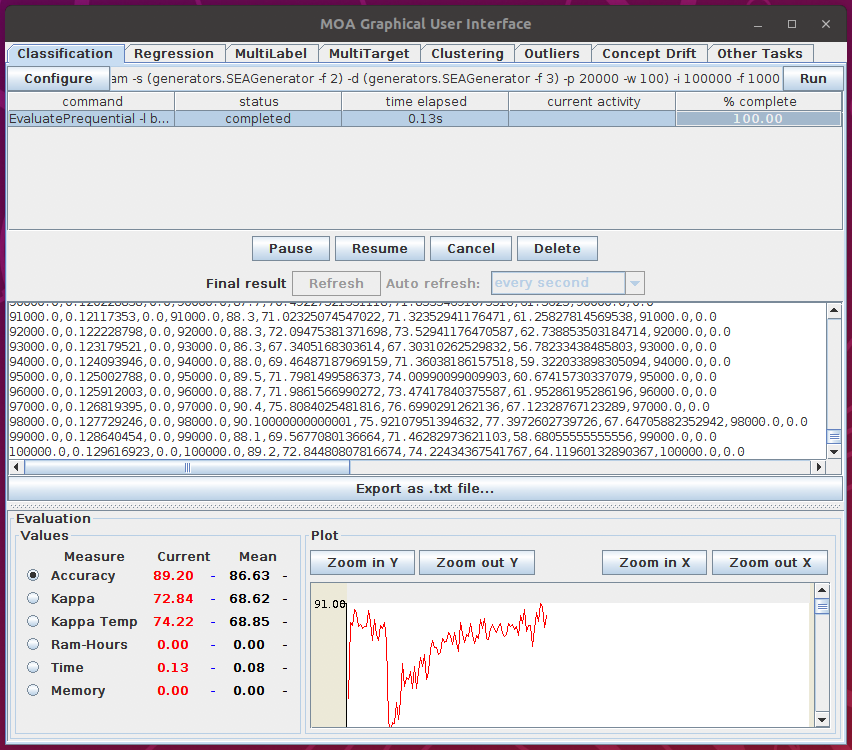
\includegraphics[width=\linewidth]{ejercicio2.png}
\end{figure}

Podemos observar que, justo cuando se produce el cambio de concepto, la precisión del modelo cae drásticamente y que, conforme se va adaptando a los nuevos datos, esta precisión se recupera.

\subsection{Ejercicio 3.}

Entrenar un modelo estático Na\"{i}ve Bayes sobre 100.000 instancias de la función 2 del generador SEAGenerator. Seguidamente, evaluarlo con un flujo de datos con desvío de concepto generado por el generador de datos SEAGenerator, con un desvío de concepto centrado en la instancia 20.000 en una ventana de 100 instancias. Para simular el desvío de concepto, hacer que el simulador genere la función -f 2 al principio, y luego la función -f 3. \\

Para solucionar este ejercicio, el comando usado en MOA es el siguiente:

\begin{lstlisting}[language=bash]
EvaluateModel -m
	(LearnModel -l bayes.NaiveBayes -s (generators.SEAGenerator -f 2) -m 100000) -s
	(ConceptDriftStream
		-s (generators.SEAGenerator -f 2)
		-d (generators.SEAGenerator -f 3)
		-p 20000 -w 100) -i 100000
\end{lstlisting}

En la línea uno entrenamos el modelo asociado a la primera parte de la pregunta. A continuación, generamos el \textit{Concept Drift}, al igual que hemos hecho en el ejercicio anterior. El resultado obtenido es el siguiente:

\begin{table}[H]
	\centering
	\begin{tabular}{rl}
		\textbf{Métrica} & \textbf{Valor} \\ \hline
		classified instances & 100000 \\
		classifications correct (percent) & 80.344 \\
		Kappa Statistic (percent) & 57.301 \\
		Kappa Temporal Statistic (percent) & 54.583 \\
		Kappa M Statistic (percent) & 39.098 \\
		model training instances & 100000 \\
		model serialized size (bytes) & 0.0
	\end{tabular}
\end{table}

Lo que sucede en este experimento es que estamos entrenando un modelo estacionario, es decir, en la primera parte de los datos, antes de que suceda el \textit{Concept Drift}. Cuando este sucede, dato que el modelo no ha sido entrenado teniéndolo en cuenta, los resultados del experimento empeoran, tal y como podemos ver en las métricas \textit{Kappa}.

\subsection{Ejercicio 4.}

¿Qué ocurriría si pudiésemos detectar un cambio de concepto y re-entrenar un modelo estacionario? El resultado no sería un modelo ``estacionario'', sino múltiples de ellos entrenados tras detectar cambio de concepto. Se pide: Evaluar, y entrenar online con el método TestThenTrain, un modelo estacionario Na\"{i}ve Bayes que se adapta (re-entrena) tras la detección de un cambio de concepto mediante el método DDM (función SingleClassifierDrift). Usar el flujo de datos del ejercicio anterior. \\

Para solucionar este ejercicio, el comando usado en MOA es el siguiente:

\begin{lstlisting}[language=bash]
EvaluateInterleavedTestThenTrain 
	-l (moa.classifiers.drift.SingleClassifierDrift -l bayes.NaiveBayes -d DDM) 
	-s (ConceptDriftStream 
		-s (generators.SEAGenerator -f 2) 
		-d (generators.SEAGenerator -f 3) 
	-p 20000 -w 100) 
-i 100000
\end{lstlisting}

El resultado obtenido es el siguiente:

\begin{figure}[H]
	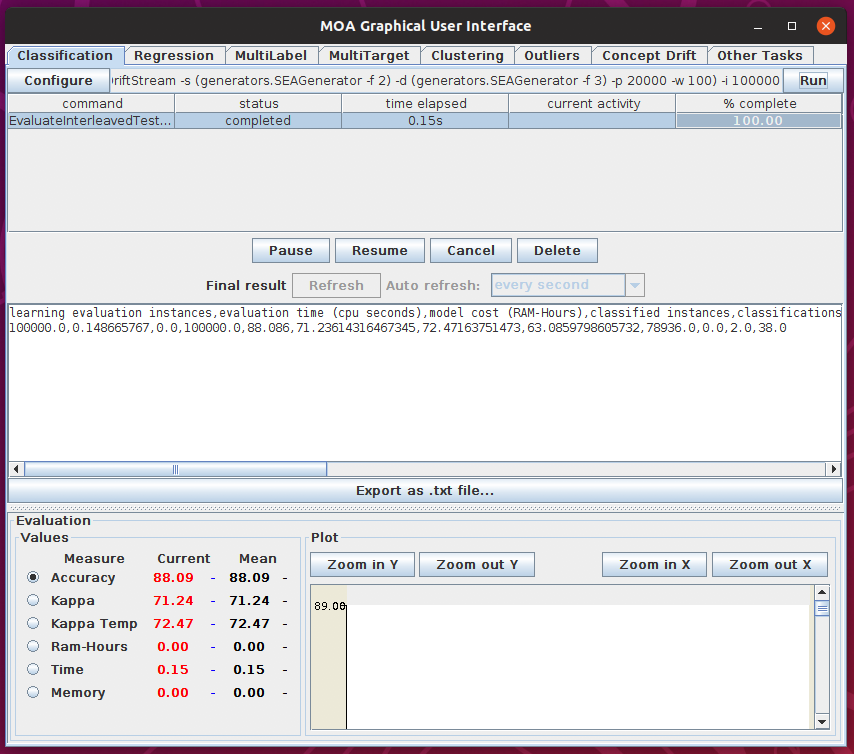
\includegraphics[width=\linewidth]{ejercicio4.png}
\end{figure}

Si construyésemos una población de resultados e hiciésemos tests estadísticos de comparación entre este modelo y el anterior:
\begin{itemize}
	\item Vemos que el porcentaje de aciertos y el estadístico Kappa mejora sustancialmente.
	\item Es el resultado esperado: Tras un cambio de concepto, un modelo estacionario deja de funcionar. Se debe reentrenar para ser usado en el nuevo contexto.
\end{itemize}
\end{document}